\section{Data structure}
\label{sec:data_structure}

\subsection{Description of the data structure}
The raw data is \textbf{only} stored in the Via Appia Linux server and there is Python script that needs to be used to generate the converted OSG data, the \textit{createosgdata.py}. The raw data directory is \textit{/home/vadata/DATA/RAW}. OSG data is stored in \textit{/home/vadata/DATA/OSG} and POTREE data is stored in \textit{/home/vadata/DATA/POTREE} (figure \ref{fig:directory_structure_overview}). 

The next subsections explores the RAW data tree in more detail and discusses how to modify and list the data in the RAW data tree.

\begin{figure}[!ht]
 \centering
 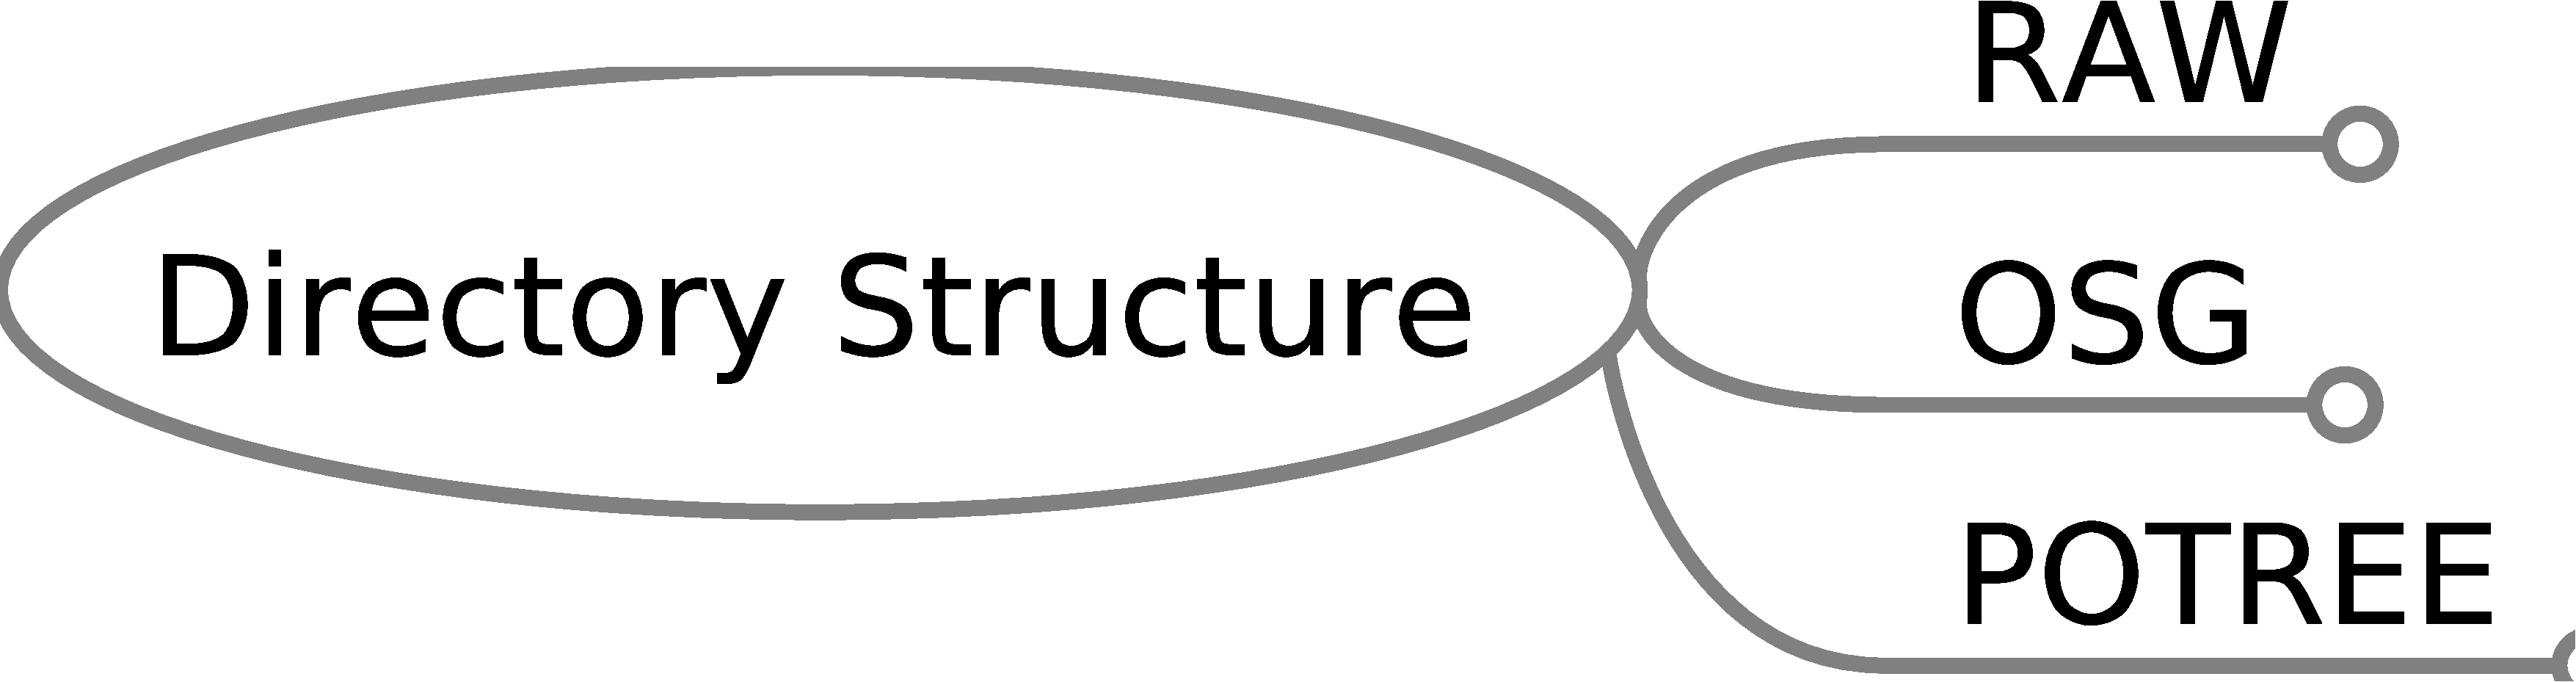
\includegraphics[width=0.4\textwidth]{fig/directory_structure_overview}
 \caption{Overview of the data structure}
 \label{fig:directory_structure_overview}
\end{figure}

\paragraph{Point clouds}
Higher resolution point clouds are stored in the subdirectories \textit{PC/BACK} and \textit{PC/SITE}, for respectively backgrounds and sites. For backgrounds, the subdirectory contains different folders with point clouds for each background. For sites, the subdirectory contains a separate folder for each site (e.g.\ \textit{PC/SITE/S162} for site 162), which in turn contain different folders for each point cloud of the site. These folders contain LAS files of different point clouds of the site. 

The LAS files contained in each site subfolder may have been pre-aligned (using CloudCompare for example). In that case the LAS file name must be \textbf{*\_ALIGNED\_\textit{BGNAME}*} where \textit{BGNAME} must be the background name (as contained in the folder \textit{PC/BACK/}).
Some point clouds generation tools store the color information in 8 bits instead of the usual 16 bits. In that case the folder name must be \textbf{*\_8BC}. The effect of having an undeclared LAS file with 8 bit color is that the converted data will be black and white. Note that these properties are cumulative, for example \textit{S162\_ALIGNED\_DRIVE\_1\_V3\_8BC} is a valid name for a folder containing a LAS file with 8 bit color information and aligned points.

\begin{figure}[!ht]
 \centering
 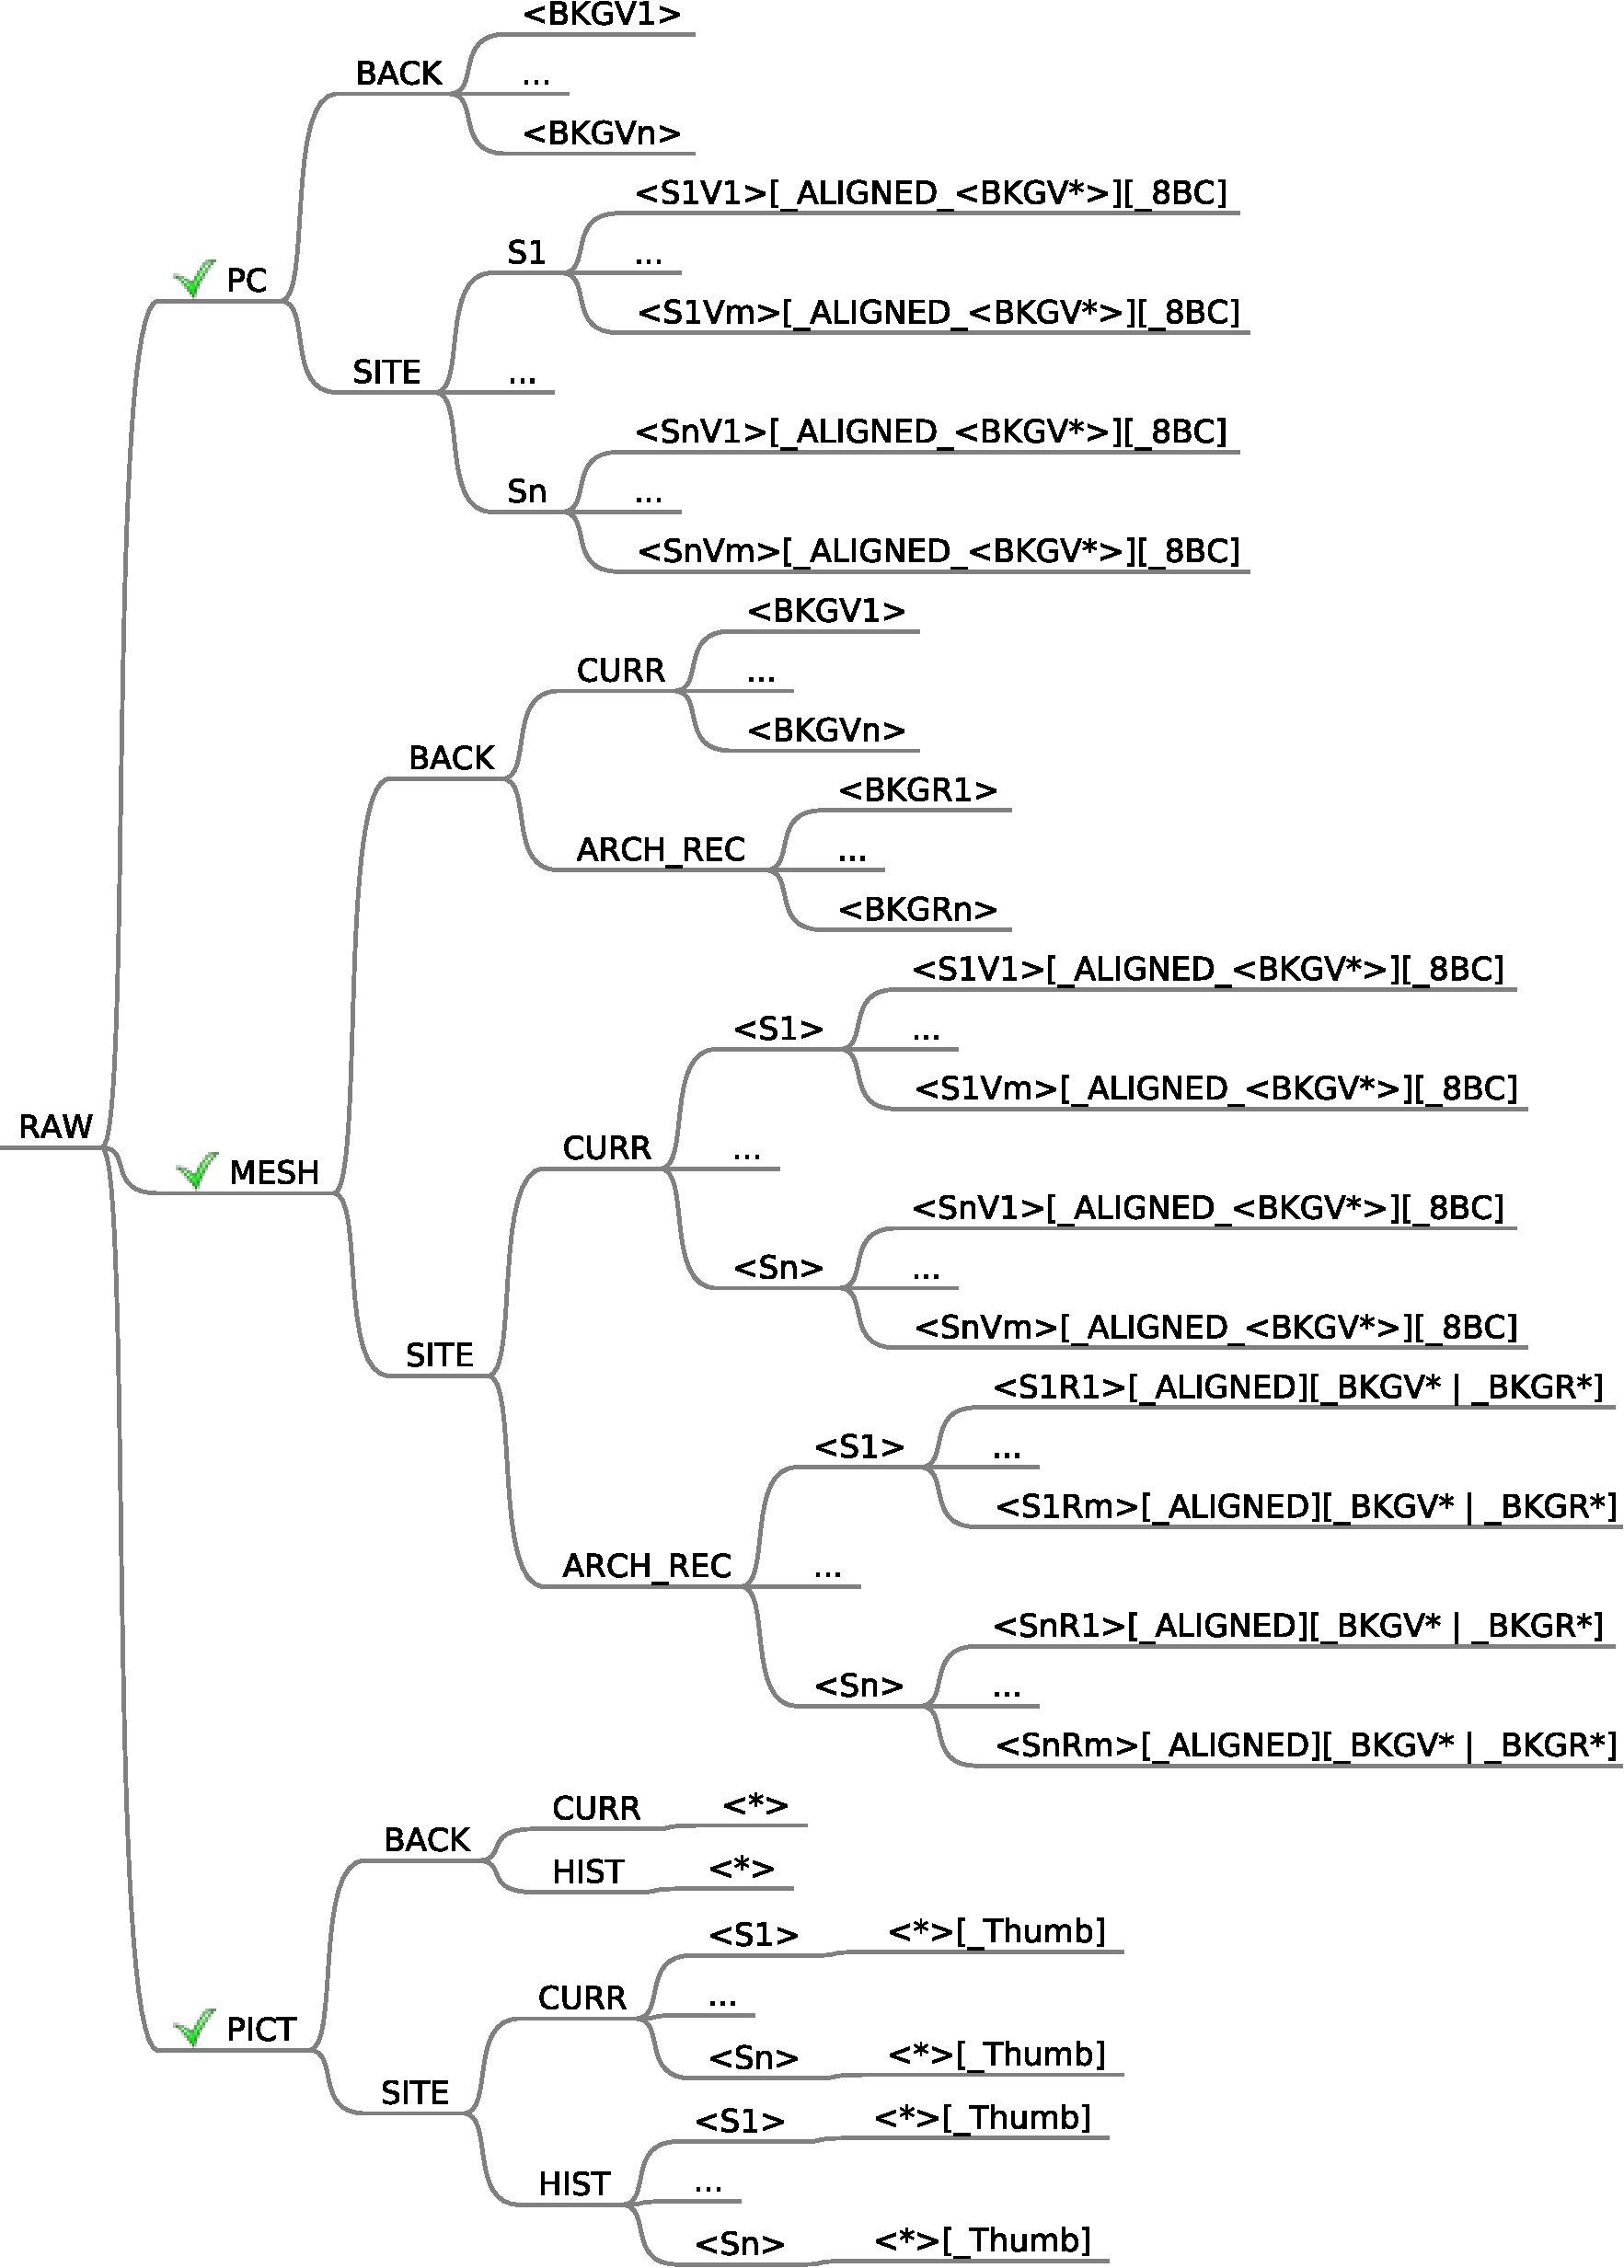
\includegraphics[width=0.95\textwidth]{fig/directory_structure_raw}
 \caption{Overview of the data structure: RAW data items}
 \label{fig:directory_structure_overview_raw}
\end{figure}

\paragraph{Meshes}
Meshes are stored in the directories \textit{MESH/BACK} and \textit{MESH/SITE}, for respectively backgrounds and sites. There are two types of meshes: (a) current  mesh representations, and (b) archeological reconstructions. For backgrounds, they are stored in respectively \textit{MESH/BACK/CURR} and \textit{MESH/BACK/ARCH\_REC}. For sites they are stored in respectively \textit{MESH/SITE/CURR} and \textit{MESH/SITE/ARCH\_REC}. For sites, each of these directories contain different folders for each site. For example the folder \textit{MESH/SITE/CURR/S162} contains mesh representations of the current state of the site 162. 

For each site there must be different folders for the several meshes. Inside these folders the files for the meshes are stored (OBJ, MTL, JPEG). For example \textit{MESH/SITE/CURR/S162} could contain two folders called \textit{162\_curr\_1} and \textit{162\_curr\_2} and each of them contain a OBJ, a MTL and several JPEG files. 

Similarly to the LAS files the meshes can also be aligned. In this case the folder name for a certain mesh must be \textbf{*\_ALIGNED\_\textit{BGNAME}*}. 

\paragraph{Pictures}
Pictures are stored in the subdirectory \textit{PICT}. Pictures can be either of a background or of a site. For both types a further subdivision is made between (a) pictures of the current state of the sites, and (b) historical pictures and paintings. These are stored in respectively \textit{PICT/BACK/CURR} and \textit{PICT/BACK/HIST} for backgrounds, or \textit{PICT/SITE/CURR} and \textit{PICT/SITE/HIST} for sites. For sites, each of these directoryes contains a separate folder for each site. For example the folder \textit{PICT/SITE/CURR/S162} contains pictures of the current state of the site 162.


\subsection{Operation on the data structure}
\subsubsection{Adding raw data items}
This section describes the script that should be used to add raw data items to the directory structure: \textit{AddRawDataItem.py}.

\begin{Verbatim}[fontfamily=courier,commandchars=\\\{\},fontsize=\footnotesize]
 usage: AddRawDataItem.py [-h] [-i DATA] -k {BACK,SITE} -t {PC,MESH,PICT} -f FILE                                                                                                     
             [-p {CURR,HIST,ARCH_REC}] [-s SRID] [--eight]
             [-l {debug,info,warning,error,critical}] [--site SITE]

Add Raw data item to the file structure.

optional arguments:
  -h, --help            show this help message and exit
  -i DATA, --data DATA  RAW data folder [default /home/pattydat/DATA/RAW]
  -s SRID, --srid SRID  spatial reference system SRID [only for MESH SITE]
  --eight               8 bit color [only for PC SITE or MESH]
  -l {debug,info,warning,error,critical}, --log {debug,info,warning,error,critical}
                        Log level

required arguments:
  -k {BACK,SITE}, --kind {BACK,SITE}
                        Type of item
  -t {PC,MESH,PICT}, --type {PC,MESH,PICT}
                        Type of data
  -f FILE, --file FILE  Input file/directory name to copy

required arguments for MESH and PICT:
  -p {CURR,HIST,ARCH_REC}, --period {CURR,HIST,ARCH_REC}
                        Period (choose from MESH:CURR,ARCH_REC;
                        PICT:CURR,HIST)

required arguments for SITE:
  --site SITE           Site number
\end{Verbatim}

\subsubsection{Removing RAW data items}
This section describes the script that should be used to remove RAW data items from the file structure: \textit{RemoveRawDataItem.py}.
\begin{Verbatim}[fontfamily=courier,commandchars=\\\{\},fontsize=\footnotesize]
 usage: RemoveRawDataItem.py [-h] -i ITEMID [-d DBNAME] [-u DBUSER] [-p DBPASS]
                            [-t DBHOST] [-r DBPORT]
                            [-l {debug,info,warning,error,critical}]

Removes a list of Raw data items and their related converted data from the
file structure.

optional arguments:
  -h, --help            show this help message and exit
  -i ITEMID, --itemid ITEMID
                        Comma-separated list of Raw Data Item Ids Raw data
                        item id (with ? the available raw data items are
                        listed)
  -d DBNAME, --dbname DBNAME
                        PostgreSQL DB name vadb]
  -u DBUSER, --dbuser DBUSER
                        DB user [default $USERNAME]
  -p DBPASS, --dbpass DBPASS
                        DB pass
  -t DBHOST, --dbhost DBHOST
                        DB host
  -r DBPORT, --dbport DBPORT
                        DB port
  -l {debug,info,warning,error,critical}, --log {debug,info,warning,error,critical}
                        Log level
\end{Verbatim}

\subsubsection{Listing raw data items}
This section describes the script that lists the RAW data items currently in the file structure: \textit{ListRawDataItem.py}.
\begin{Verbatim}[fontfamily=courier,commandchars=\\\{\},fontsize=\footnotesize]
 usage: ListRawDataItem.py [-h] [-i ITEMID] [-d DBNAME] [-u DBUSER] [-p DBPASS]
                          [-t DBHOST] [-r DBPORT]
                          [-l {debug,info,warning,error,critical}]

List the Raw data items that are in the DB.

optional arguments:
  -h, --help            show this help message and exit
  -i ITEMID, --itemid ITEMID
                        List the Raw Data Item Ids related to a list of items
                        (comma-separated) [default list all raw data items]
  -d DBNAME, --dbname DBNAME
                        PostgreSQL DB name vadb]
  -u DBUSER, --dbuser DBUSER
                        DB user [default $USERNAME]
  -p DBPASS, --dbpass DBPASS
                        DB pass
  -t DBHOST, --dbhost DBHOST
                        DB host
  -r DBPORT, --dbport DBPORT
                        DB port
  -l {debug,info,warning,error,critical}, --log {debug,info,warning,error,critical}
                        Log level
\end{Verbatim}
